\documentclass[11pt, oneside]{article}   	% use "amsart" instead of "article" for AMSLaTeX format
\usepackage{geometry}
\usepackage[linesnumbered]{algorithm2e}
\geometry{letterpaper}
\usepackage{graphicx}
\usepackage{amsmath, amsthm, amssymb}
\usepackage{parskip}
\usepackage{titlesec}
\usepackage{enumerate}
\graphicspath{ {images/} }

\newtheorem*{theorem}{Theorem}
\newtheorem*{lem}{Lemma}
%SetFonts
\titleformat{\paragraph}
{\normalfont\normalsize\bfseries}{\theparagraph}{1em}{}
\titlespacing*{\paragraph}
{0pt}{3.25ex plus 1ex minus .2ex}{1.5ex plus .2ex}
\title{CS340 - Project Description and Analysis}
\author{Yutong Li, Tianming Xu, Jiaping Wang}
\date{\today}							% Activate to display a given date or no date

\begin{document}
\maketitle

\section{Description}
\subsection{Notation}
Let $S$ be the set of students, with $|S|=s$. Each student will have a list of class requests, so let $l_{s_i}$ to represent the $i^{th}$ student's list of class requests. We denote the set of teachers by $P$ and its cardinality by $|P|=p$. Let $C$ be the set of classes, and so we have $|C|=c$ classes. Denote the set of classrooms by $R$, with $|R|=r$, and the set of time slots as $T$, with $|T|=t$. 
\subsection{Algorithm Description}
Given $S, P, C, R, T$, we determine a class schedule with following rule: schedule as many students as possible into each class in decreasing order of the class' popularity, defined by the number of students hoping to take this class. \par 
Start off by sorting the classes in decreasing order of popularity. Sort the classrooms in decreasing order of capacity. \par
Then, we can begin pairing classes with classrooms and time periods. Starting with the most popular class $c_1$, we try scheduling this class in the biggest classroom $r_1$ during its first available time slot $t_1$. Find the teacher $p_1$ who teaches $c_1$. If $p_1$ has no conflict during this time, put the class-room-time combination into the final schedule. Otherwise, add the (room, time) combination as a skipped slot and move on to the next slot. Once this class is scheduled, mark both the teacher and classroom as unavailable during this time period. Repeat this process for the next most popular class in the next time slot, except that if there are previously skipped slots, we try scheduling the class to the skipped slot(s) first. Otherwise, always try scheduling the class in the largest available classroom during its earliest available time slot, checking for conflicts with teacher. Keep doing so until either all classrooms are filled at all times, or all $2m$ classes has been scheduled.\par
After all class time and location are settled for all classes, we proceed to select students for each class in the same order. Starting with the most popular class, as long as there are seats available in the classroom, we randomly select a student from those who signed up for this class. If the student has no conflict at the same time, pair the student with the class. If the student has a conflict, remove him/her from the pool and select another one. Repeat the process until either all seats are filled or all prospective students are considered.
\subsubsection{Haverford Extension}
In order to schedule classes before pre-registration data is available and to more accurately reflect real-life situations at Haverford, we consider the following additional constraints:
\begin{enumerate}
\item There are six core classes for each major. Thus, it is more important to schedule these classes before others.
\item Consider the number of majors and minors in each department to determine the relative popularity of classes.
\item Intro-level classes are likely to have larger size than higher-level classes.
%\item Assign popularity to time slots in order to schedule popular/important classes at more popular times.
\item Different time slots are allowed to have overlapping times.
\item Teachers may have personal time conflicts.
\item Some classes have a lab session, which must be scheduled during a consecutive 2.5-3 hour time slot rather than the usual 1-1.5 hour lecture times that are spread out on different days.
\end{enumerate}
%describe our constraints and explain why they are well-reasoned.
\par To determine a popularity rating without preregistration data, we predict the popularity of a class based on past enrollment data, the number of majors in its department, its class level, and whether a class is core. The number of enrolled students in Spring 2014 is used as a reference value for expected class size. We also predict popularity based on the number of majors and minors in each department. Classes from popular departments, like Computer Science, are highly demanded each semester. Therefore, making sure that these classes are offered However, we also want to schedule core classes first because these are classes students must take to fulfill they graduation requirement, whereas distributional requirements and electives can be fulfilled by choosing any class within a certain range. Furthermore, giving priority to core classes when scheduling allows students with less popular majors to finish their majors. Otherwise, if only popular classes are scheduled, these students might never have the opportunity to take any class in their majors. 
Besides, we want to consider professors' personal time conflicts to better simulate the actual conflicts. For instance, some professors are fathers/mothers, so probably they cannot teach a class between 8:00-10:00 AM or 3:00-5:00 PM because of their children's school schedule. The last constraint adds lab session, which is very common for natural sciences classes in our college. Furthermore, we also schedule fine arts classes during lab times, since studio work usually require longer class time. 
%talk about how we implement the constraints
\par From the csv file containing Spring 2014 enrollment data, we can get rooms, time slots, classes, department, class level, and instructor information. Since we don't have the information about whether a class is a core class for some major, we choose the two classes with most enrolled students from each of $100$-, $200$-, and $300$-levels in every department and assign these are core. In addition, every class that has department number "WRPR", i.e. is a writing seminar, are also labeled as core, since there must be enough writing seminars for first-years to complete their writing requirement. For professor's personal conflicts, we randomly assign $0-5$ unavailable time slots for each professor. 
\par For lab scheduling, we separate the set of time slots into two parts: lecture time and lab time, the former usually takes 1 - 1.5 hour in two or three days, and the latter takes 2.5 to 3 hours in one sitting. 
% Need work here
When scheduling classes, we first consider all lectures in sorted order based on their predicted popularity. If a class being scheduled has lab, we immediately schedule the lab after the schedule for lecture is finalized. % We still have a queue to store the time or room that is not satisfied for the current class, we will set next class to the time or room in queue if it is available for that class. Since this time we have labs, if a class has lab, we will assign the lab into the schedule right after we schedule this class. There is another function schedule lab, which works similarly as the one we schedule lectures.\\
Follow this design, we are able to simulate the real-life situation to make a proper schedule before we can get the enrollment information from students.
\section{Pseudocode}
\begin{algorithm}[H]
\SetKwFunction{Schedule}{Schedule}
\SetKwProg{Fn}{Function}{}{}
\Fn{\Schedule{S, P, C, R, T}}{
Sort $C$ in decreasing order of popularity.\\
Sort $R$ in decreasing order of capacity.\\
Compute the maximum number of classes that can be scheduled: $max\gets rt$.\\
Let $k=0$ be the class we're scheduling.\\
Let $i=0$ be the first available time slot in the largest available room.\\
$skippedSlots\gets$ empty\\
 \While{$i < \min \{2m, max\}$}{
 	\uIf{$skippedSlots$ is empty}{
	        	\While{ teacher $P_{C_k}$ who teaches $C_k$ is not available during $T_i$}{
        			Put $i$ in $skippedSlots$\\
			$i\gets i+1$}
		Schedule class $C_k$ in room $R_{i}$ at time $T_{i}$.}
        	\uElse{
		\While{$skippedSlots$ is not empty }{
	   		Pop $j$ from $skippedSlots$\\
	   		\uIf{ teacher $P_{C_k}$ has a conflict with the skipped slot}{
	    			Push the slot back to $skippedSlots$}
	   		\uElse{
				Schedule class $C_k$ in room $R_{i}$ time $T_{j}$.\\
				\textbf{break}
			}
		}
		\uIf { $skippedSlots$ is empty and $C_k$ hasn't been scheduled}{
			Try scheduling $C_k$ at slot $i$, checking conflicts with teacher
		}
        	}
	$k\gets k+1$
	}


\For{each scheduled class}{
	\While {the classroom is not full and not all potential students are checked}{
		Choose a random student from the pool of prospective students
	\uIf{ student has another class at this time}{
		Go to the next student}
	\uElse{
		Schedule this student for the class}
	}
}
\Return $Schedule$
}
\end{algorithm}

\section{Time Analysis}
\subsection{Data Structure}
The class requests of each student can be stored as an array. Constructing the lists in $S$ takes $O(s)$ and accessing a student's class choices takes $O(1)$. Furthermore, it takes $O(c)$ to assign each class a popularity. Sorting classes by popularity with the standard quicksort requires $O(c\log c)$.\par
The instructor information $P$ for classes can be stored in an array indexed by the classes. Thus initialization of $P$ takes $O(p)$, and retrieving the teacher of a given class $C_k$ takes $O(1)$. Similarly, classroom capacities can be stored in an array. Construction of $R$ takes $O(r)$ and sorting $R$ takes $O(r\log r)$.\par
Information about teachers' assignments can be stored in an array indexed by the teachers, which takes $O(p)$ to initialize. Each time a class is scheduled, append the time $t_i$ to the teacher's assignments. Because each teacher teaches at most two classes, the size of each teacher's assignments cannot exceed $2$. Thus, checking whether $P_{C_k}$ has conflict during time $T_i$ takes $O(1)$.\par
The skipped slots due to teachers' time conflicts can be stored in a FIFO queue. Therefore, pushing a slot into the queue, checking if it's empty, as well as popping its first element can be done in constant time. Since each teacher teaches at most two classes, each teacher can have at most $1$ conflict and so construction requires $O(p)$.\par
To store the final schedule, we can create an array of size $rt$, where the $i$-th value in the array indicates the class assignment in room $\lfloor i / t\rfloor$ during time $(i\mod t)$. Initialization of the array takes $O(rt)$. Accessing or changing each value can be done in $O(1)$.\par
Consider the time for choosing students for each class already been scheduled. Since in optimal situation all students and all class can be scheduled, thus in sum there're $4n$ students to be scheduled. The choosing students algorithm is based on built-in random selection, and thus takes $O(1)$ for each student. Further more, for each student, there's a need to check whether the class time conflicts with this student's existing schedule, which takes $O(1)$. In total, choosing students have a $O(s)$ complexity.


\subsection{Time Complexity} % Redo this. Use the new notation
%Add time analysis for looping over skippedSlots in basic. Add extension 
Using the data structures described above, we know that, in total, initialization requires \[s+c+c\log c+p+r+r\log r+p+rt+s = O(c\log c+r\log r +rt+s).\] By construction of the algorithm, the {\it while} loop terminates when all classrooms are $filled$ during all time periods or $2m$ classes are scheduled. Therefore, the nested {\it while} loops runs $\min(rt, 2c)$ times. Therefore, the overall time complexity of the algorithm is 
\begin{align*}
T(input) &= O(c\log c+r\log r +rt+s)+O(\min(rt, 2c))\\
& = O(s+r\log r+c\log c +rt)
\end{align*}
Since $s$ dominates, we can say the time complexity of the algorithm is $O(s)$.

\section{Proof of Correctness}
\underline{\textit{Proof of Termination.}} By time analysis we know the {\it while} loop runs at most $\min(xy, 2m)$ times. Each time a class is scheduled, $k, j$ are incremented by $1$. Furthermore, each time $j$ reaches $x$, $i$ is also incremented by $1$. Therefore, one of the loop preconditions will be violated as $i$ and $k$ keeps increasing. Hence, the algorithm terminates.

\underline{\textit{Proof of Validity.}}
We claim that each class-room-time combination added to the final schedule is valid. \\ \par
\begin{lem}No two classes are scheduled in the same classroom at the same time.\end{lem}
\begin{proof}Suppose for a contradiction that $C_k$ and $C_l$ are both scheduled into the same slot, $(R_j, T_i)$. Without loss of generality, suppose $l>k$ in the sorted list of classes. By execution of the algorithm, we know $C_k$ gets added into the schedule before $C_l$. Then, when $C_k$ is added, we increment $i$ by $1$ so that all classes after $C_k$ don't get assigned to the same time. When $i$ exceeds $x$, we set $i$ back to $0$ and increment $j$. Therefore, by the time $C_l$ gets scheduled to $(R_j', T_i')$ we have:
\[ \begin{cases} j'\geq j \\i'>i& \text{,if } $j=j'$ \end{cases}\]
Therefore, it is impossible to have $j=j'$ and $i=i'$ at the same time. Hence, there does not exist two classes that conflict with each other. \end{proof}
\begin{lem}No teacher is teaching two classes at the same time.\end{lem}
\begin{proof}Suppose there is a teacher $p$ who is scheduled to teach $C_k$ and $C_l$ at the same time. Without loss of generality, suppose $C_k$ is more popular than $C_l$. Thus, when $C_l$ gets scheduled, $C_k$ has already been scheduled in room $R_j$ at time $T_i$. Thus, $occupied[p]$ will contain $T_i$.\par
However, before the schedule of $C_l$ is added, we check for $occupied[p]$. Since $T_i$ is in $occupied[p]$, $C_l$ will never be scheduled during the same time $T_i$. Therefore, we conclude this is impossible. 
\end{proof}
Since the returned schedule satisfies the two lemmas above, it does not contain any conflicts and hence is a valid schedule.
\section{Discussion}
Possible solution might come from following categories:  dynamic programming, graph algorithm, recursion, naive algorithm, and greedy algorithm. 
\par First consider dynamic programming and recursion. Both algorithms involve ideas of dividing and conquering. However, in scheduling problem, since rooms can only be used by single class in each time slots, dividing students into different groups and arrange schedules respectively is trivial. Thus, dynamic programming and recursions cannot apply to this problem.\par
Then suppose graph algorithm can tackle this problem. According to the property of all graph algorithm, there must exist a way to transform given inputs into a graph data model, such as DAG. In any graph model, limits are interpreted as weights of edge, while objects constrained by limit are interpreted as vertices. Consider following: since the performance of algorithm depends on how many classes students can take, consequently, students are defined as vertices. Furthermore, the order of schedule has no effect on the performance, thus the graph is undirected. As stated above, limits are interpreted as edges, and according to the description of the problem, room size, teachers, time slots are all restrictions the algorithm needs to fulfill. Nevertheless, each edge can only pair up with a single restriction. Hence, an undirected graph cannot represent scheduling problem.\par
Naive algorithm aims to enumerate all possible schedules and compares their performance in order to get an optimal output. Yet, restrictions exist among given input, and thus requires large amount of collisions check. As a result, naive algorithm cannot given an acceptable time complexity.\par
% not optimal
Greedy algorithm guarantees optimal result for each iteration, in this case the number of class students can take. Accordingly, greedy algorithm always needs to ensure the most popular class is correctly arranged. In other words, the most popular class need to pair up with the largest room in order to get as most students as possible enrolled.
\par What is more, limits also exist on room size and time slots. Owing to the fact that a room can only be arranged to one time slot at a time, algorithm needs to schedule classes not only regarding room size but also guarantee that time conflict will not occur among popular classes.
\par Complications come mainly from restrictions on teachers and time slots. A simple corner case is that a teacher teaches two classes $c_i,c_j$, $c_i$ is more popular in $c_j$, but the algorithm automatically arrange them into the same time slot. A natural way to solve this conflict is to simply skip that time slot and move downward. However, this will result in an empty room at that time slot. To make full use of each room, a skipped room marker is needed. Whenever the algorithm skipped a room, the marker will keep track of that room, and arrange the next popular to that time slot.
\par To conclude, greedy algorithm will give an near-optimal result and can be done in an acceptable time complexity.
 
 \section{Experimental Analysis}
 \subsection{Time Analysis:}
As we stated above, our expectation on run time is $O(s)$. The result of our experiment shows that it indeeds have a linear run time. The algorithm is run on input generated by $\text{make\_random.pl}$ with different number of students. Specifically, input is generated with 50 rooms, 360 classes, 10 time 
slots fixed and the variable is number of students ranged from 50 to 5000. For each set of parameters, we generated 5 different input. Then for every set, we compute an average time, and create a graph where the x-axis represents the number of students and y-axis represents run time. After curve fitting, we find that it's linear. To validate this mathematically, we compute the $\frac{\text{number of students}}{\text{run time}}$ for each set of input. The result shows that most of the ratio lies around $800$ and the standard deviation is $38.57$. Observe that the main deviation occurs when the student size is small, $ie$ when there're 1000 students. We trust that this deviation is caused by the less frequent occurrence  of conflicts when there're fewer students. We also repeat the experiment with 20 time slots, and curve fitting generates a similar result.
\subsection{Quality Analysis}
Within each set of input, our algorithm shows a stable performance. For instance, for 3000 students, 8 times slots, 20 rooms, 160 classes, the standard deviation on $student$  $preference$  $value$ is 95.5, with an average of 9623 total enrollment. Furthermore, the most significant stand deviation occurs when there're 5000 students, which we think is caused by the increasing occurrence of conflicts in students' schedule. 
\\Then consider the performance on $student$ $preference$ $value$ for sets of input where number of rooms, classes time slots fixed and student size is the variable. We choose the lower bound of $student$ $preference$ $value$ for each set of input. First, consider there're 10 time slots, 50 rooms, 360 classes. For this set of input, our student size ranges from 1000 to 5000. Computing $\frac{\text{student preference value}}{\text{best Case Student Value}}$, we find that for different size of students, the ratio is almost the same, with a standard deviation of 0.0009. Thus, the average of these ratios can represent the performance of our algorithm on these set of input. With an average of $0.86308125$, our algorithm can arrange $86\%$ of students for their preferred classes.\\ \\Then we repeat the experiment on different sets of input with 8 time slots, 20 rooms, 160 classes, and again student size ranges from 1000 to 5000, but this time with more realistic parameters. For these set of data, we apply the same analysis strategy and get an average of $0.8023$ ratio. This ratio means that for 8 time slots, 20 rooms, 160 classes, we can arrange $80\%$ of students for their preferred classes.\\
\\We think the difference between the two different ratios result from different number of time slots, and rooms. For the first set of data, there're 10 time slots, and 50 rooms, indicating more slots for classes and also a less occurrence of time conflicts. Under such a circumstance, our algorithm can arrange more classes and will thus generate a better performance.
\section{Time Analysis: Haverford Extensions}
\subsection{Data Structure}
\\Also, for one of the extension, we're considering overlap among time slots. In our basic version, checking room conflicts and teachers' time conflicts only takes $O(1)$ since there're no overlaps we can check by simply testing whether there that time has already been taken. However, even a time slot is not taken, it still might cause a conflict because it may overlap with a time that's already taken. Thus, for each class we assigned, the algorithm needs to traverse list of taken time slots of current room and that of current teacher, which in worst case might traverse all time slots, that is $O(t)$. Also, overlapping time slots will also affect the process of enroll students into classes. Similarly, for each students, when assigning them to classes, algorithm needs to check whether there's a time conflict in students' personal schedule by traversing it. However, since each student can only take a limited number of classes, implying checking time conflicts for one students takes $O(1)$ time. Thus, choosing students has a $O(s)$ time complexity.\\
\\In order to deal with skipped time slots that only work for lab session, we're using another FIFO queue to store skipped time slots. Since we're having time slots overlap, it is possible that a teacher has time conflicts with all time slots, so construction requires $O(t)$ time.\\
\subsection{Time Complexity}
Aside from assigning lectures, we also need to assign labs which follows exactly the same process of assigning lectures. Therefore, assigning labs can be represented as modifying number of classes, which our main loop iterates on. Since class can have at most one lab, thus adding a constant less than $c$ won't change the iteration of our main loop. In total, for initialization we have: 
\\\hspace*{30mm}$c\log c + p + r + r\log r+ p + rt + s = O(c\log c + p + rt + s)$
\\Similarly, the main $while$ loop will terminate when all classes are scheduled or all time slots and rooms are taken, thus there will be $min(rt, c)$ iterations. As we mentioned above, due to overlapping time slots, each loop takes $O(t)$ to check conflicts, hence:
\\\hspace*{30mm}$T(input) =  O(c\log c + p + rt + s) + O(min(c, rt)\times t)$
\\\hspace*{46mm}$=O(c\log c + p + rt^2 + s)$\\
Since $s$ dominates, we can say the time complexity of the algorithm is O(s).
\subsection{Quality Analysis}
%==================Figure 1===================
\begin{figure}[H]
\centering
\begin{tabular}{ |c||c|c|c|c|c|c| } 
 \hline
 Number of students & $1000$  & $2000$ & $3000$ & $4000$ & $5000$\\ 
  \hline \hline 
 Optimal Student Preferences Value & $(3131)$ & $(6136)$  & $(8485)$ & $(9489)$ & $(10365)$ \\
  \hline
Worst Case Student Preferences Value& $(1166)$ & $(2476)$ & $(6931)$ & $(8036)$ & $(5107)$ \\ 
 \hline
Ave. Student Preferences Value& $(2465.9)$ & $(5461)$ & $(7992)$ & $(8603)$ & $(8951)$ \\
 \hline
 Ave. Time Taken & $(1.9531)$ & $(1.88398)$ & $2.2616)$ & $(2.71231)$ & $(2.44185)$ \\
 \hline
\end{tabular}
\caption{Performance table} %Change this name
\end{figure}
%=======quality analysis
Comparing to the performance shown in basic version, the Haverford extension version doesn't have a very stable performance. In Haverford extension version, we only consider the performance on $student$ $preference$ $value$ for sets of input where number of rooms, classes time slots fixed and student size is the variable, because the time slots and classrooms will be imported from $HaverfordEnrollmentData$ file. We choose the lower bound of $student$ $preference$ $value$ for each set of input. First, consider there are 58 time slots( some of them overlap with each other), 47 rooms, 268 classes. For this set of input, our student size ranges from 1000 to 5000. The preference lists of students are generated by a new random input generator and the number of class each student wants to take varies between 2 - 7, considering student might want to take class in Bryn Mawr or Swarthmore. Computing $\frac{\text{student preference value}}{\text{best Case Student Value}}$, we find that for different size of students, the ratio decreases after the size of students reaches 3000. The average of these ratios can represent the performance of our algorithm on these set of input. We found that when student size is 1000 - 3000, the performances of these three tests are $0.8219666667$ (size 1000), $0.9101666667$ (size 2000) and $0.888$ (size 3000), which means that our algorithm can arrange $82\%$ of students for their preferred classes, if there are 1000 students, and can arrange $91\%$ of students for their preferred class, when there are 2000 students. Though our algorithm has a very promising performance on small input size, when size of student is larger than 3000, the total number of students enrolled in class does not increase much. So the performance here is $0.7222$ (4000) and $0.5967333333$ (5000) and we can see a obvious compromise of performance after 3000 students.
\\We think the possible reason of this compromise of performance is that the fixed available time slots and classrooms, especially the classrooms, limit the performance of our algorithm when we apply it on large size input. We checked the total capacity of all rooms in Haverford is 1153, with average capacity of 24 people per rooms, and for 5000 students, the reasonable guess of total population of all classes is 15000, which requires a lot of valid time slots to fit in. When there is not enough spot to assign class, our algorithm will terminate and return the schedule. Hence, we believe our algorithm's performance will be much better if the we can have more classrooms with larger capacity. 
\\We also test our algorithm by the original student preference list parsed from 2014 HaverfordEnrollmentData. There are 1177 students and the performance of this test is $81\%$, it is similar to our result in testing 1000 students. 
%==================Figure 2===================
\begin{figure}[H]
\centering
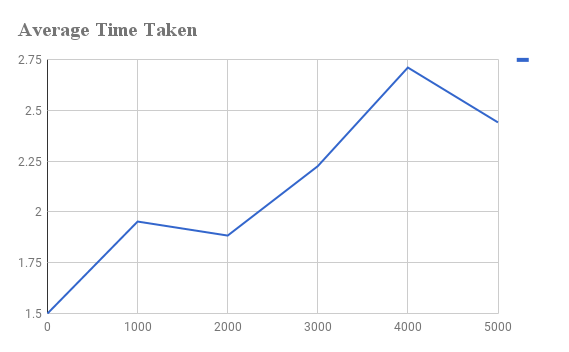
\includegraphics[scale =.6]{chart}
\caption{Average Time Taken by our algorithm}
\label{timechart}
\end{figure}
%=================Time Analysis=============
In our haverford extension version we no longer sort courses based on popularity only, instead, algorithm will assign weight to classes based on course level, major and other information in $O(1)$ time as well. Since we need to assign all courses and sort them, thus it takes $O(c+c\log c) \to O(c\log c)$ time, and getting enrollment information from 2014 data takes $O(s)$ time. From Figure \ref{timechart}. we can see that even we have no student, we still need to do all these preparations in 1.5 seconds. Then we find that the rate of change of the line is linear-time. The reason that it vibrates when the size of input increases is that the time spent on assigning student depends on the quality of random generated input. If the input has a lot of conflicts,  we need to check time conflict much more than a good quality input file. Here, the overall quality of input with size 1000 is slightly bad and one with size 5000 is slightly better than expected. Through Figure \ref{timechart}, we can see our algorithm's running time increases in linear time.

\section{Recommendation and Improvement}
During the experiment of our program, we have three recommendations to current registration office. Firstly, it would be better if registration office is able to get the popularity of each department and make schedule based on the popularity of department. For example Computer Science are highly demanded each semester. Therefore, making sure that these classes are offered in big classrooms is very important. Otherwise, student might not be able to get in those classes. Secondly, it would be better for registration office to get the core courses list from each department, because these are classes students must take to fulfill they graduation requirement. Besides the core of each department, they should also consider distributional requirements and electives can be fulfilled by choosing any class within a certain range.  Hence, we want to schedule these important and popular classes first into big classrooms. The last recommendation is that it will be better to have a priority value for each time slots. Students prefer class time to be between 10 am and 3 pm so they can get up not that early and have no conflict with their varsity training. So do professor for different personal conflicts. If registration office can assign these time slots to big classrooms with popular classes, students and professor might have less conflicts with their personal life, which will be able to make more students assigned to the classes they want to take.
\\In our implementation, we still have several thoughts to improve our current scheduling algorithm but because of the approaching due date, we are not able to implement them but we would like to share our thoughts here. The first improvement is to add multiple lab sessions when we assign lab session. In our current implementation, we can only assign one lab for each course which requires lab, but some departments, say, chemistry and biology, may require more than one lab sessions. It will be better to consider this situation. The second improvement is to have a more selective check-time-conflict function. In our current implementation, we only check whether two class times conflict with each other, instead of knowing which class conflict with which. It will be better to get this information because we can assign scientific classes at the same time as the time assigned to social science or humanity classes, as students take them should be fairly different, especially in high level classes. So it is possible for student to have less conflicts in his class list if we do so. These improvements are probably very promising, so we might try to further improve our program in these directions in the future.

\end{document}

